%%%%%%%%%%%%%%%%%%%%%%%%%%%%%%%%%%%%%%%%%%%%%%
\section{Photon Detector Electronics and DAQ}\label{sec:pds-elec-daq}

%%%%%%%%%%%%%%%%%%%%%%%%%%
\subsection{Readout}

Scintillation light from LAr comes from the two different excited 
states with lifetimes of about 6 ns and 1.6 $\mu$s. 
Only a limited amount of light is collected by this system, so we 
assume the electronics must be designed to collect the light 
from both excited states. A summary of the general requirements 
for the system, including initial requirements from a 
physics performance perspective, are given in Table~\ref{tab:fee_req}.
%
\begin{table*}[ht]
\centering
%\vspace{4mm}
\begin{tabular}{| l | l |} \hline
 Performance Parameter       & Target   \cr   \hline
 Time Resolution                   & Better than 30 ns wrt event time zero ("t0")      \cr  \hline
 Charge Resolution               & 0.25\% photo-electron equivalent                     \cr \hline
 Dynamic Range                   & $\sim$ x10 better than detector (1000:1)          \cr \hline
 Linearity                               & Sufficient to resolve 1 photo-electron signals   \cr    \hline
 Multi-Hit Capability              & Sufficient to measure Triplet (late) Photons          \cr   \hline
 Dead Time                           & Live up to 2 drift times either side of beam spill          \cr    \hline
 Bias Control                        & 0.1 V resolution up to 30 V per channel  \cr    \hline
 Calibration                          & On-board Charge Injection  \cr    \hline
 Timing                                 & Events time-stamped using NO$\nu$A Timing or equivalent syst.  \cr    \hline
\end{tabular}
\caption{\label{tab:fee_req} Physics Requirements for the Photon Detector Electronics.}
\end{table*}
%
The plans for the electronics for the photon detection subsystem 
include a baseline design with several options 
that remain R\&D activities.   

In the baseline plan, there are no front-end electronics in the cold volume.  
Instead, the un-amplified signals from the SiPMs 
are transmitted to outside the cryostat on cables for processing and digitization.
%, as shown in Fig.~\ref{fig:fig-e-1}.  
%There are advantages and disadvantages to this approach.  
The advantages are that the infrastructure required for inside the cryostat is 
reduced (power, data cables, precision clocks, data protocols, etc.); reliability is 
improved (no single-point failures of multi-channel 
devices inside the cryostat); serviceability and accessibility to the front-end 
electronics are improved; and the need to develop cold 
electronics, possibly a custom ASIC, is eliminated.  
Generally, the baseline 
design favors simplicity, reliability and reduced R\&D time and costs, and also 
meets the performance requirements of the electronics.  

We have designed and built a 
custom module for receiving SiPM signals, and performing signal 
processing in the front-end as preprocessing for trigger and DAQ.  
The module is called the SiPM Signal Processor (SSP).  
An SSP consists of 12 readout channels packaged in a self-contained 
1U module.  
Each channel contains a fully-differential voltage amplifier and a 
14-bit, 150 MSPS analog-to-digital converter (ADC) that 
digitizes the waveforms received from the SiPMs.  
The front-end amplifier is configured as fully-differential with high common-mode 
rejection, and receives the SiPM signals into a termination resistor that 
matches the characteristic impedance of the signal cable. 
Currently there is no shaping of the signal, since the SiPM response 
is slow enough relative to the speed of the digitization to obtain 
several digitized samples of the leading edge of the pulse for the determination of signal timing.  

The digitized data is stored in pipelines in the SSP, for up to $\sim$ 13 $\mu$s.  
The processing is pipelined, and performed by a Xilinx Artix-7 
Field-Programmable Gate Array (FPGA).  
The FPGA implements an independent Data Processor (DP) for each channel.  
The processing incorporates a leading edge discriminator for detecting events
and a constant fraction discriminator (CFD) for sub 
clock timing resolution.  
Because the FPGA is programmable and accessible, it is possible to explore 
different data processing algorithms and techniques, and even customize the 
readout for a given type of event (supernova for example.)  
A picture of the module is shown in Fig.~\ref{fig:PD_fig-e-2}.  
A block diagram of the system is shown in Fig.~\ref{fig:PD_fig-e-3}.
%Fig. xx3.  Picture of the SSP module.
%
\begin{cdrfigure}[SSP Photograph]{PD_fig-e-2}{Picture of SSP module.}
  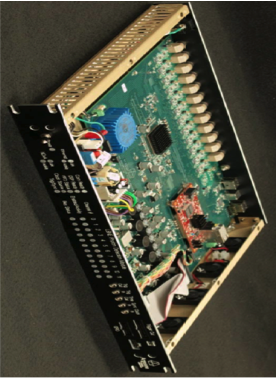
\includegraphics[angle=90,width=0.5\textwidth]{PD_fig-e-2.png}
\end{cdrfigure}
%\begin{figure}[h]
%  \centering
%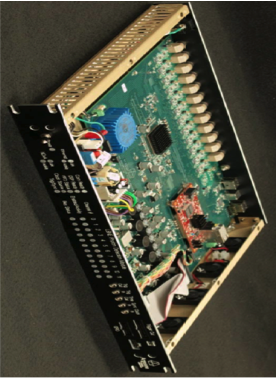
\includegraphics[angle=90,width=10cm,height=5cm]{PD_fig-e-2.png}
%\caption{Picture of the SSP module.}
%\label{fig:fig-e-2}
%\end{figure}
%
%Fig. xx2.  Block diagram of the SSP.
%
\begin{cdrfigure}[SSP Block Diagram]{PD_fig-e-3}{Block diagram of the SSP Module.}
  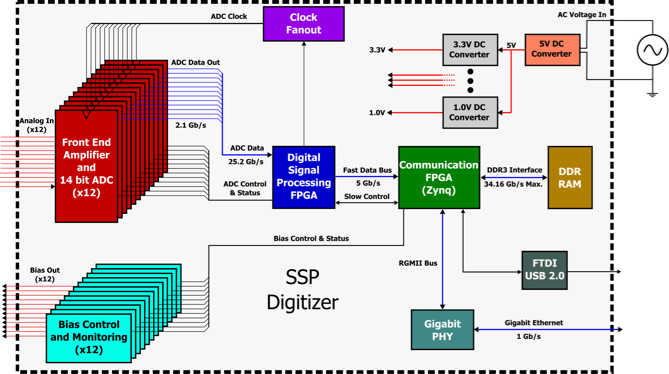
\includegraphics[angle=90,width=0.5\textwidth]{PD_fig-e-3.png}
\end{cdrfigure}
%\begin{figure}[h]
%  \centering
%\includegraphics[angle=0,width=12cm,height=7cm]{fig-e-3.png}
%\caption{Block diagram the SSP module.}
%\label{fig:fig-e-3}
%\end{figure}
%
In the simplest mode of operation, the module can perform waveform capture, 
using either an internal trigger or an external trigger.  
Up to 2046 waveform samples may be read out for each event.  When waveform 
readouts overlap the device can be configured to offset, 
truncate or completely suppress the overlapping waveform.  
Pile-up events can also be suppressed.  

As an alternative to reading full waveforms, the DP can be configured to 
perform a wide variety of data processing algorithms, 
including several techniques for measuring amplitude, and also timing of 
the event with respect to a reference clock.  
All timing and amplitude values are reported in a compact event record.  
Each data processing channel stores up to 340 event records when not storing waveforms.  

Generally, the SSP performs pipelined processing.  
The module has been designed to support several different triggering schemes, 
including self-triggered, use of an external trigger, or use an 
external gate to readout all events within a time-window.  
In order for the events measured in the photon detector to be matched up 
with the corresponding events in the TPC, the front-end electronics 
attaches a timestamp to the data as it is acquired.  
The timestamp is unique, and has a correspondence with the timestamps in 
the TPC electronics processing.  
The timestamp in the SSP is applied to the event data as it is digitized, 
and becomes part of the data as the processing proceeds.  
In the case where zero-suppression and data sparsification are used, 
the timestamp on accepted data remains intact.  
To achieve this, the TPC and PD electronics must be synchronized, 
including timestamp counter resets, and a known and stable calibration between 
the corresponding timing resolution of the ADC conversion in the two systems.  
The electronics has been designed to support a full interface to the NOvA 
timing system, which is the baseline timing system for the experimental prototypes.

A Xilinx Zynq FPGA, onboard the MicroZed system-on-module, handles the 
slow control and event data transfer.  
The SSP has two parallel communication interfaces; USB 2.0 and 10/100/1000 Ethernet.  
The 1 Gb/s Ethernet supports full TCP/IP protocol.  
The module includes a separate 12-bit high-voltage DAC for each channel to 
provide up to 30 V of bias to each SiPM.  
The module also feature charge injection for performing diagnostics and linearity 
monitoring, and also voltage monitoring.

In tests to date, the SSP is capable of measuring single photo-electron signals 
coming from the SiPMs over a cable length of 30 meters when the SiPMs are 
operated at LAr temperatures.  
The timing resolution of the signals has been measured to be better than 3 ns.  
The full-differential signal processing in the front-end circuitry 
is important in achieving this result.
 
The SSP is self-contained in that it receives 60 Hz, 120V power, and has internal 
linear and DC/DC power supplies for generating the DC voltages needed for the 
instrumentation, as well as the bias voltage for the SiPMs.  
The SSP is packaged in a 1U, rack-mountable package. For the 35-ton prototype, 
the racks are located near the ports on the top of the cryostat.  

The system has been implemented and operated with the DUNE 35 ton prototype 
(describe, show an example waveform).
%
In the 35-ton prototype, each SiPM signal was transmitted on an individual 
shielded twisted-pair cable fitted with individual LEMO-style connectors.  
The bias voltage was coupled onto the signal cable, using AC-coupling on 
the receiving end to measure the SiPM signal.  
The use of high-quality cable with point-to-point connections between an 
individual SiPM inside the cryostat and the front-end electronics residing 
outside the cryostat, combined with good differential signal processing on 
the receiving end, enabled the demonstration of the principle that single 
photo-electron signals could be measured accurately without the need for 
cold electronics.  
In order to significantly reduce the complexity with the cable plant, 
the following approach are being pursued for the protoDUNE:  
\begin{itemize}
\item Ganging together of several SiPM outputs from a given PD detector 
into one output cable.  
This increases the detector capacitance, affects the pulse shape, and
could spoil the timing resolution of the measurement.  
Also, the SiPMs may have to be preselected, since there will be only one 
bias voltage for three devices, and it may be important to match the 
over-voltage characteristics.  
Studies are in progress to find a compromise between data precision and 
cabling issues. 
One approach is to add a cold pre-amplifier if the ganging together of several 
SiPMs result in performance that is too degraded to meet specifications.  
The infrastructure requirements (cables, connectors, power, cold performance, 
reliability, mechanical mounting, etc.) would have to be considered.

\item Use of multi-conductor, individually shielded pair cable.  
A candidate cable containing four individually-shielded twisted pairs has been 
identified and tests are in progress.  
The cable is in Teflon jacket, which should be acceptable for use in LAr.

\item Use of mass-terminated connectors.  
Several candidate connectors for use with the cable described above are being pursued.
\end{itemize}

The baseline plan assumes that three SiPM signals can be ganged 
together into one readout channel. 
By using the multi-conductor cable with four twisted pairs, this 
results in one cable per PD consisting of 12 SiPMs, which reduces the 
cable plant by $\sim$ x10 compared to that used in the 35 ton detector.  
The cost of the connectors also decreases by $\sim$ x10.  
Lastly, the ease in making connections at the flange board will be improved 
by the use of a mass-terminated connector.      


%%%%%%%%%%%%%
\subsubsection{DAQ interface}


%%%%%%%%%%%%%%%%%%%%%%%%%
\subsection{QC Procedures}
